\documentclass{article}
\usepackage{graphicx} % Required for inserting images
\usepackage{booktabs} % Para mejor calidad en las tablas
\usepackage{amsmath}  % Para soporte matemático si se necesita
\usepackage{multirow} % Para usar \multirow en tablas
\usepackage[utf8]{inputenc}
\usepackage[T1]{fontenc}
\usepackage[spanish]{babel}
\usepackage[margin=2.5cm]{geometry}
\usepackage{amsmath}
\usepackage{amssymb}
\usepackage{pgfplots}

\setlength{\parindent}{0pt}

\title{
    \textbf{Teoria de Valuacion de Activos Financieros} \\ 
    Resumen y notas de la clase
    \\
    \small Bibliografia: Investments - Bodie 13th edition
}
\author{Ezequiel Telias}
\date{}

\begin{document}

\maketitle

\section{Efficient Diversification}
La decision de inversion pude verse como un top-down process. Primero, alocacion de capital entre un portafolio riesgoso y activos
libre de riesgo. Luego, la alocacion de activos ente el portfolio riesgoso a traves de diferentes tipos de instrumentos (Acciones locales, internacionales
bonos a largo plazo). Finalmente, seleccion de securities de un activo individual entre diferentes tipos de instrumentos (Apple, Microsoft entre activos de US).

\subsection{Diversification and Portfolio Risk}
Suponiendo que un portfolio se compone por un activo, se puede decir que las dos principales fuentes de incertidumbre son, 
el riesgo que viene de factores de la economia en general y el riesgo especifico de la firma.
Ejemplificando una diversificacion ingenua, suponemos que tenemos un portfolio dividido en dos activos, ExxonMobil y Microsoft. Existen dos riesgos especificos
de la empresa, por ejemplo, si baja el precio del petroleo, podemos deducir que bajara el precio de ExxonMobil pero esto tambien puede ayudar a que el precio de las 
tecnologicas suban generando dos efectos de offsetting y estabilizacion de los retornos del portfolio. 
\\

Concluyendo, si diversificamos para tener una cantidad grande de activos, igualmente no podemos mitigar el riesgo del mercado.
\\

\textbf{Insurance principle:} Cuando todos los riesgos son especificos de la firma, la diversificacion puede reducir el reisgo a niveles arbitrariamente bajos. 
La razon es porque estos son independientes entre si, y la exposicion a cualquier fuente de riesgo puede ser reducida a nivieles casi nulos. Entonces, la reduccion de riesgo 
bajo propagacion hacia muchos riesgos independientes es llamada principio de insurance.

\subsection{Portfolios of Two Risky Assets}
Se introduce el termino de diversificacion eficiente, done se construyen portfolios con el menor riesgo y mayor nivel de retorno. 
\\

Se tienen dos activos con riesgo, un bono de deuda a largo plazo llamado D y una accion de equity llamado E. Se denota $w_E$ como el peso de E y siendo que tenemos dos activos,
el peso de D sera 1 - $w_E$. Entonces la tasa de retorno de este portfolio $r_p$ se calcula multiplicando el peso por la tasa
de retorno de cada security.

\[
\begin{aligned}
r_p = w_D \cdot r_D + w_E \cdot r_E
\end{aligned}
\]

El retorno esperado del portfolio es similar siendo:
\[
E(r_p) = w_D \cdot E(r_D) + w_E \cdot E(r_E)
\] 

A diferencia, de los retornos esperados, no alcanza con multiplicar el peso del activo en el portfolio
 con su varianza. El calculo real seria el siguiente, pero al tener la covarianza de cada activo con si mismo igual a su varianza
  se puede simplificar. Entonces la varianza del porftolio es la suma de los pesos de los activos en el portfolio multiplicado por su covarianza.

 \[
 \sigma_p^2 = w_D w_D \operatorname{Cov}(r_D, r_D) + w_E w_E \operatorname{Cov}(r_E, r_E) + 2 w_D w_E \operatorname{Cov}(r_D, r_E)
\]

\[
\sigma_p^2 = w_D^2 \sigma_D^2 + w_E^2 \sigma_E^2 + 2 w_D w_E \operatorname{Cov}(r_D, r_E)
\]


Se intoruce el termino de bordered matrix, que es la matriz de covarianza con los pesos del portfolio de cada activo.
Supongamos un portafolio con dos activos \( A \) y \( B \), con pesos \( w_A \) y \( w_B \), y la siguiente matriz de covarianzas:

\[
\begin{bmatrix}
\sigma_A^2 & \operatorname{Cov}(A, B) \\
\operatorname{Cov}(B, A) & \sigma_B^2 \\
\end{bmatrix}
\]

La bordered covariance matrix sería:

\[
\begin{array}{c|cc}
 & w_A & w_B \\
\hline
w_A & \sigma_A^2 & \operatorname{Cov}(A, B) \\
w_B & \operatorname{Cov}(B, A) & \sigma_B^2 \\
\end{array}
\]

\bigskip

Para calcular la \textbf{varianza del portafolio} \( \sigma_p^2 \), se multiplica cada elemento interno de la matriz 
por los pesos correspondientes en su fila y columna, y se suman todos los productos:

\[
\sigma_p^2 = \sum_i \sum_j w_i w_j \cdot \operatorname{Cov}(r_i, r_j)
\]

\bigskip

\textbf{Ejemplo numérico:}

Supongamos:
\begin{itemize}
    \item \( w_A = 0.6 \), \( w_B = 0.4 \)
    \item \( \sigma_A^2 = 0.04 \), \( \sigma_B^2 = 0.09 \)
    \item \( \operatorname{Cov}(A, B) = 0.03 \)
\end{itemize}

Entonces:

\[
\sigma_p^2 = (0.6)^2 \cdot 0.04 + (0.4)^2 \cdot 0.09 + 2 \cdot (0.6)(0.4) \cdot 0.03 = 0.0432
\]

\bigskip

Este enfoque es útil especialmente cuando se trabaja con matrices grandes o en hojas de cálculo, ya que permite visualizar fácilmente cómo los pesos afectan la varianza total del portafolio.

\bigskip

La covarianza tambien puede ser computada con el coeficiente de correlacion:
\[
\operatorname{Cov}(r_D, r_E) = \rho_{DE} \cdot \sigma_D \cdot \sigma_E \tag{7.6}
\]
\begin{itemize}
  \item \( \rho_{DE} \): correlación entre los activos \( D \) y \( E \)
  \item \( \sigma_D \), \( \sigma_E \): desvíos estándar de los activos \( D \) y \( E \)
\end{itemize}

\[
\sigma_p^2 = w_D^2 \cdot \sigma_D^2 + w_E^2 \cdot \sigma_E^2 + 2 w_D w_E \cdot \sigma_D \cdot \sigma_E \cdot \rho_{DE}
\]

\textbf{Que pasa cuando un activo tiene un peso menor a 0?}
Un peso $w_E$ negativo, implica que el activo fue vendido short, y reinvertido en otro fondo. 

\subsection{The Markowitz Portfolio Optimization Model}
\subsubsection{Security Selection}
Primero, se van las combinaciones disponibles de riesgo retorno para activos de riesgo. Luego, identificaremos el 
portfolio optimo buscando las ponderaciones que resultan en la CAL (Linea de asignacion de capital) mas empinada. 
Finalmente, elegimos un porfolio combinando activos libre de riesgo con el portfolio optimo.

El primer paso es buscar la frontera de minima varianza de los activos libre de riesgo. Esta frontera es 
 un grafo de los puntos de menor varianza por retorno esperado.
 
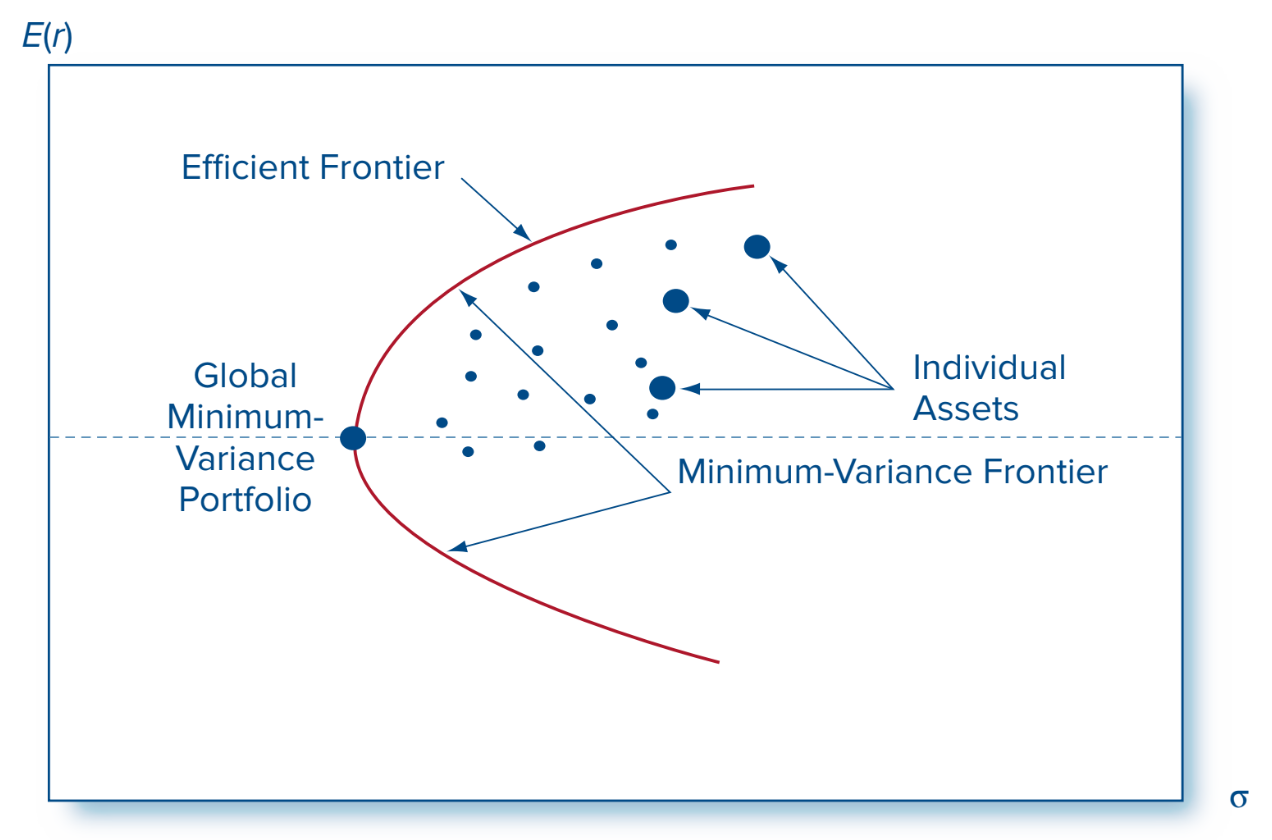
\includegraphics[width=15cm, height=10cm]{./img/7_minima_varianza.png}

Se puede ver que

\begin{itemize}
  \item Todos los activos individuales se encuentran dentro de esta frontera, al menos cuando permitimos construccion
de portfolios con short selling.
  \item Todos los potfolios que estan dentro de la frontera de minima varianza desde el minimo global tienen el mejor ratio de riesgo-retorno y se llama frontera eficiente de activos riesgoso
  \item Todos los activos por debajo de la curva tienen una opcion con mejor retorno. Entonces esta parte de la curva es ineficiente.
\end{itemize}

\newpage
La segunda parte de la optimizacion incluye los activos libre de riesgo. Como antes, buscamos la CAL con el Sharpe ratio mas alto (o la pendiente mas empinada).
Esta CAL se genera a partir del portfolio optimo P, tangente a la frontera eficiente. Esta CAL domina todas las posibles alternativas dentro de la frontera. Entonces P 
es el portfolio optimo.

\bigskip
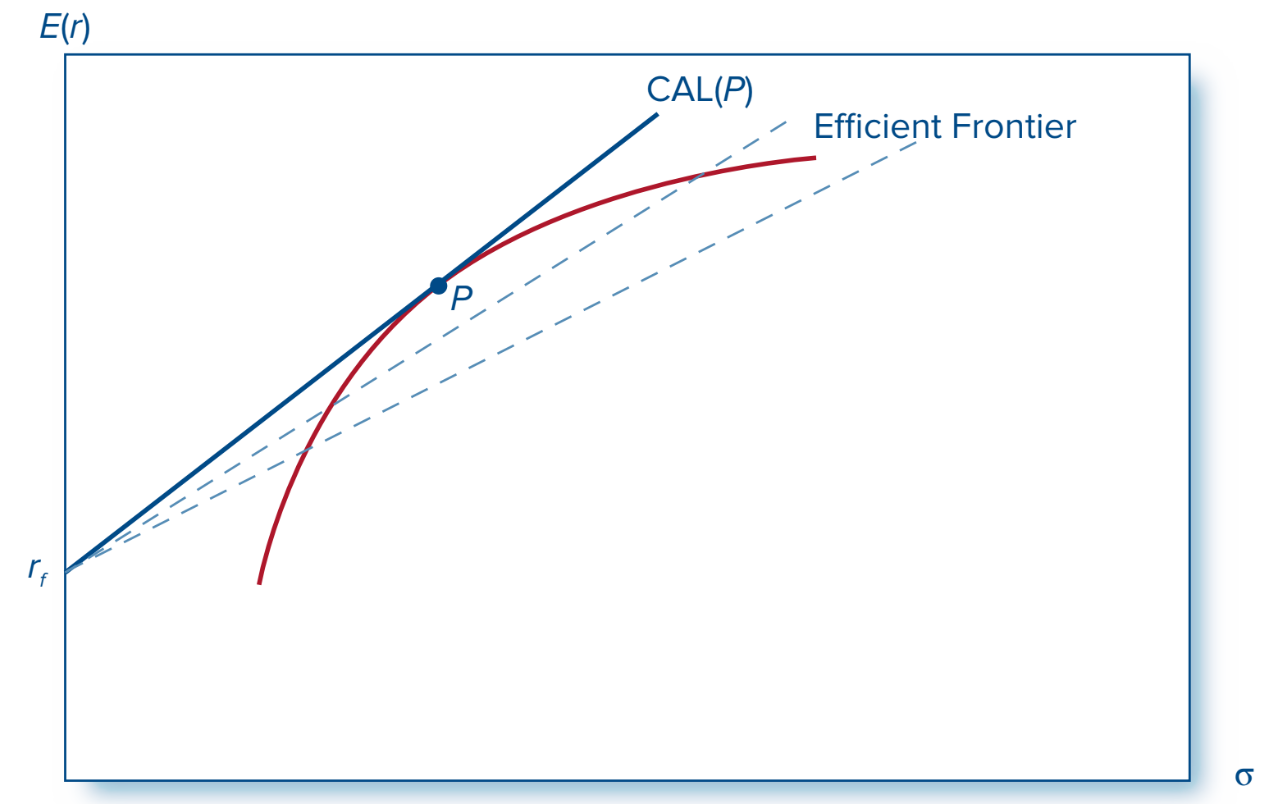
\includegraphics[width=15cm, height=10cm]{./img/7_minima_varianza_sharpe.png}

Finalmente, el inversor toma una decision entre el portfolio con riesgo P y los activos libre de riesgo.
\bigskip

El administrador del porfolio ahora tiene un n estimados de retornos esperados $E(r_i)$ y un $n\times  n$ estimados de matiz de covarianza.
en donde la diagonal son estimados de las varianzas $\sigma^2_i$. Teniendo todos los datos se concluye en las siguientes formulas.

\begin{equation}
E(r_p) = \sum_{i=1}^{n} w_i \, E(r_i)
\end{equation}

\begin{equation}
\sigma_p^2 = \sum_{i=1}^{n} \sum_{j=1}^{n} w_i w_j \, \text{Cov}(r_i, r_j)
\end{equation}

\subsection{Capital Allocation and the Separation Property}
En el paso dos incluimos los activos libres de riesgo. Se traza la CAL hasta que llegamos al portfolio P, que es el punto tangente
 desde F a los portfolios de la frontera de eficiencia.  Otra manera de encontrar el portfolio P optimizado es maximizando el Sharpe Ratio.

Se supone que el manager de portfolio ofreceria el mismo risk portfolio a todos los clientes sin importar su aversion al reisgo. Donde entra,
la alocacion de capital. Donde los clientes con mas aversion al riesgo elegiran activos libre de riesgo con mayor ponderacion por sobre el portfolio riesgoso.
Este resultado se llama \textbf{Separation Property}.

\subsection{Risk Sharing versus Risk Pooling}
TBA
\subsection{Time Diversification}
TBA

\end{document}